\newcommand{\hmwkTitle}{Homework 8}
\newcommand{\hmwkDueDate}{Thursday, March 3, 2016}
\newcommand{\hmwkHeaderTitle}{ICCS206 Discrete Mathematic: Homework 8}
\documentclass{article}

\usepackage{fancyhdr}
\usepackage{amsmath}
\allowdisplaybreaks
\usepackage{amsthm}
\usepackage{amsfonts}
\usepackage{tikz}
\usepackage[plain]{algorithm}
\usepackage{algpseudocode}
\usepackage{enumitem}
\usepackage{graphicx}
\usepackage{hyperref}

\usetikzlibrary{automata,positioning}

%
% Basic Document Settings
%

\topmargin=-0.45in
\evensidemargin=0in
\oddsidemargin=0in
\textwidth=6.5in
\textheight=9.0in
\headsep=0.25in

\linespread{1.1}

\pagestyle{fancy}
\lhead{\hmwkAuthorName}
\chead{} % empty
\rhead{\hmwkHeaderTitle}
\cfoot{\thepage}

\renewcommand\headrulewidth{0.4pt}
\renewcommand\footrulewidth{0pt}

\setlength\parindent{0pt}

%
% Homework Details
%

\providecommand{\hmwkTitle}{Homework}
\providecommand{\hmwkDueDate}{TBD}
\providecommand{\hmwkClass}{ICCS206 Discrete Mathematic}
\providecommand{\hmwkClassTime}{Section\ 1}
\providecommand{\hmwkClassInstructor}{Pakawut Jiradilok}
\providecommand{\hmwkAuthorName}{\textbf{Jiraroj Wiruchpongsanon (6781617)}}
\providecommand{\hmwkHeaderTitle}{\hmwkClass:\ \hmwkTitle}

%
% Title Page
%

\title{
    \vspace{2in}
    \textmd{\textbf{\hmwkClass:\ \hmwkTitle}}\\
    \normalsize\vspace{0.1in}\small{Due\ on\ \hmwkDueDate}\\
    \vspace{0.1in}\large{\textit{\hmwkClassInstructor\ \hmwkClassTime}}
    \vspace{3in}
}

\author{\hmwkAuthorName}
\date{}

\renewcommand{\part}[1]{\textbf{\large Part \Alph{partCounter}}\stepcounter{partCounter}\\}

%
% Helper Commands
%

\newcounter{partCounter}
\newcommand{\solution}{\textbf{\large Solution}}

\newtheorem*{theorem}{Theorem}

\theoremstyle{remark}
\newtheorem*{remark}{Remark}

\begin{document}

\maketitle
\newpage


\section*{Problem 1: Coin-Toss Conspiracy}
Sam, May, and AJ Piti challenge Zaza to a split-the-pool coin-toss game where everyone bets 6 Baht per turn.
\begin{enumerate}[label=\arabic*.]
    \item Evil Plan 1: Sam and AJ always bet opposite results while May bets randomly. What is Zaza's expected profit/loss per turn?
    \item Use linearity of expectation to compute the combined expected return of (Sam + May + AJ Piti).
    \item Evil Plan 2: Suppose Zaza agrees to bet first each turn. Propose a better strategy for the trio and compute Zaza's expected profit/loss per turn under that strategy.
\end{enumerate}

\medskip
\solution

\begin{enumerate}
    \item for plan 1, we fix Zaza's bet to H (as if zaza bet T, the probability tree is symmetry --- so only half the tree is enough), sam and aj would pick the opposite side to zaza every turn (so, we just bemind of this, for zaza's net calculation), and may just do random pick (say with the probability of $\frac{1}{2}$ for each H and T). we can draw the probability tree as

\begin{center}
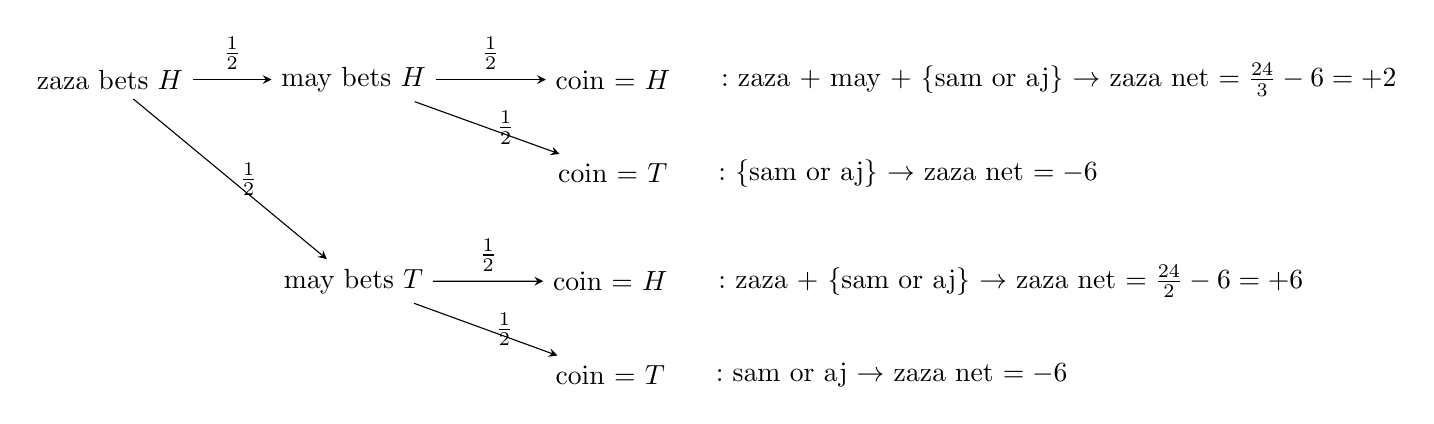
\begin{tikzpicture}[>=stealth, node distance=12mm, scale=0.95]
\node (r) {zaza bets $H$};
\node[right=10mm of r] (mH) {may bets $H$};
\node[below=20mm of mH] (mT) {may bets $T$};
\draw[->] (r) -- node[above] {$\tfrac12$} (mH);
\draw[->] (r) -- node[right] {$\tfrac12$} (mT);

  \node[right=14mm of mH] (cHH) {coin = $H$};
  \node[below=7mm of cHH] (cHT) {coin = $T$};
  \draw[->] (mH) -- node[above] {$\tfrac12$} (cHH);
  \draw[->] (mH) -- node[right] {$\tfrac12$} (cHT);

  \node[right=14mm of mT] (cTH) {coin = $H$};
  \node[below=7mm of cTH] (cTT) {coin = $T$};
  \draw[->] (mT) -- node[above] {$\tfrac12$} (cTH);
  \draw[->] (mT) -- node[right] {$\tfrac12$} (cTT);

    \node[right=4mm of cHH] {$:$ zaza + may + \{sam or aj\} $\rightarrow$ zaza net $= \frac{24}{3}-6 = +2$};
    \node[right=4mm of cHT] {$:$ \{sam or aj\} $\rightarrow$ zaza net $= -6$};
    \node[right=4mm of cTH] {$:$ zaza + \{sam or aj\} $\rightarrow$ zaza net $= \frac{24}{2}-6 = +6$};
    \node[right=4mm of cTT] {$:$ {sam or aj} $\rightarrow$ zaza net $= -6$};

\end{tikzpicture}
\end{center}

now we just read off the leaves of the tree and weight them by their probabilities:
\[
E\text{(zaza)} = \tfrac14\cdot(+2) + \tfrac14\cdot(-6) + \tfrac14\cdot(+6) + \tfrac14\cdot(-6) = \boxed{-1\ \text{baht/turn}}
\]

    \medskip
    \begin{center}
    \rule{0.3\linewidth}{0.2pt}
    \end{center}
    \medskip

\item the linearity of expectation for any random variables $A,B,C$ is
\[
    E(A+B+C) = E(A) + E(B) + E(C)
\]

        in this case (plan 1), the winner set never is empty, so there's no money lost from the table (as someone always win), so
\[
E(\text{sam}+\text{may}+\text{aj}) = E((\text{sam}+\text{may}+\text{aj}+\text{zaza}) - \text{zaza}) = 0 - E(\text{zaza}) = \boxed{+1\ \text{baht/turn}}.
\]

    \medskip
    \begin{center}
    \rule{0.3\linewidth}{0.2pt}
    \end{center}
    \medskip

\item have two of the trio follow zaza, and one bet opposed to her. using the same representatoin approach, we get

  \begin{center}
  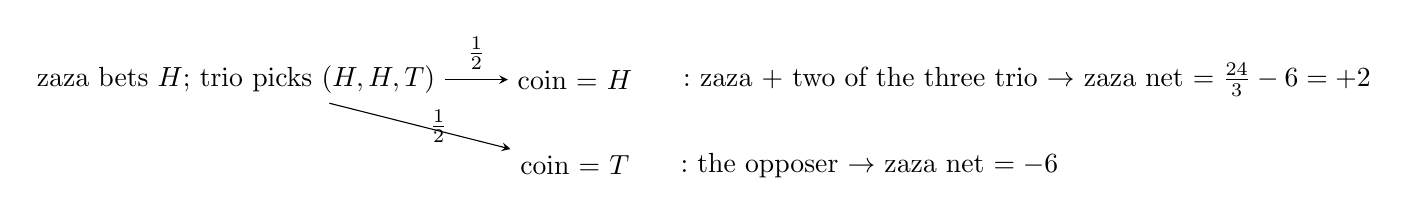
\begin{tikzpicture}[>=stealth, node distance=16mm, scale=0.95]
  \node (r) {zaza bets $H$; trio picks $(H,H,T)$};
  \node[right=8mm of r] (cH) {coin = $H$};
  \node[below=6mm of cH] (cT) {coin = $T$};
  \draw[->] (r) -- node[above] {$\tfrac12$} (cH);
  \draw[->] (r) -- node[right] {$\tfrac12$} (cT);

  \node[right=4mm of cH] {$:$ zaza + two of the three trio $\rightarrow$ zaza net $= \frac{24}{3}-6 = +2$};
  \node[right=4mm of cT] {$:$ the opposer $\rightarrow$ zaza net $= -6$};
  \end{tikzpicture}
  \end{center}

  therefore
  \[
  E(\text{zaza}) = \frac12\cdot(+2)+\frac12\cdot(-6)=
  \boxed{-2\ \text{baht/turn}}
  \]
  \end{enumerate}

\vspace{1em}
\hrulefill

\section*{Problem 2: Dice Game}
You pick a number from 1--6 and roll three fair, independent dice.
\begin{itemize}
    \item If your number never appears, you lose 1 Baht.
    \item If it appears once, you win 1 Baht.
    \item Twice yields 2 Baht.
    \item Thrice yields 4 Baht.
\end{itemize}
\begin{enumerate}[label=\arabic*.]
    \item Compute the expected profit/loss and decide if you should play.
    \item Compute the variance of your profit/loss.
    \item Now tape the three dice together so they always show the same number. What is the expected profit/loss?
    \item What is the variance in the taped-dice case?
\end{enumerate}

\medskip
\solution

\begin{enumerate}
    \item we let $X$ be our profit/loss in baht, for the independent-dice case, on each die the probability that your chosen number appears is $\frac{1}{6}$ and the probability that it does not appear is $\frac{5}{6}$

        \vspace{1em}

    let $K$ be the number of times our chosen number shows up among the three dice, and as there's only two choice,
    \[
    K\sim \mathrm{Binomial}(3,\tfrac16).
    \]

    so the probabilities are
    \[
    P(K=0)=\left(\frac56\right)^3=\frac{125}{216},
    \]
    \[
    P(K=1)=\binom31\left(\frac16\right)\left(\frac56\right)^2=\frac{75}{216},
    \]
    \[
    P(K=2)=\binom32\left(\frac16\right)^2\left(\frac56\right)=\frac{15}{216},
    \]
    \[
    P(K=3)=\left(\frac16\right)^3=\frac{1}{216}
    \]

    and the return for each K's value are, 

    \[
    X=
    \begin{cases}
    -1,& K=0,\\
    1,& K=1,\\
    2,& K=2,\\
    4,& K=3.
    \end{cases}
    \]

    now, we just add the weight to those probabilities as 

    \[
    E(X)=(-1)\frac{125}{216}+(1)\frac{75}{216}+(2)\frac{15}{216}+(4)\frac{1}{216}
    \]

        and the expacted gain per pay is $\boxed{E(X)=-\frac{2}{27}\text{ baht}}$ per play --- as it's negative, you loss money, so \boxed{\text{it's not so wise to play the game}}. 

    \medskip
    \begin{center}
    \rule{0.3\linewidth}{0.2pt}
    \end{center}
    \medskip

    \item to find the variance, we use this theorem of

    \[
    \mathrm{Var}(X)=E(X^2)-[E(X)]^2 
    \]

    we already know $E(X)$, so we only need to compute $E(X^2)$ as

    \begin{align*}
        E(X^2)&=(-1)^2\frac{125}{216}+(1)^2\frac{75}{216}+(2)^2\frac{15}{216}+(4)^2\frac{1}{216} \\
        &=\frac{125+75+60+16}{216} \\
        &=\frac{276}{216}=\frac{23}{18}
    \end{align*}

    hence, 

    \begin{align*}
        \mathrm{Var}(X) &= \frac{23}{18}-\left(-\frac{2}{27}\right)^2\\ &= \boxed{\frac{1855}{1458}}
    \end{align*}

    \medskip
    \begin{center}
    \rule{0.3\linewidth}{0.2pt}
    \end{center}
    \medskip

    \item as the three dice are taped together, making them always show the same face, there are only two possibilities, illustrate by a probability tree as

\begin{center}
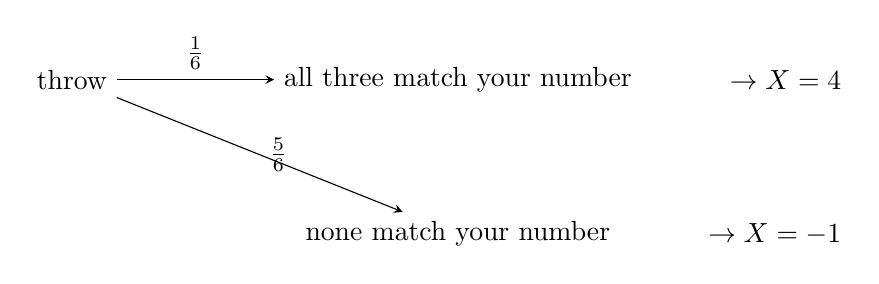
\begin{tikzpicture}[>=stealth, node distance=14mm, scale=0.95]
\node (r) {throw};
\node[right=20mm of r] (w) {all three match your number};
\node[below=14mm of w] (l) {none match your number};

\draw[->] (r) -- node[above] {$\tfrac16$} (w);
\draw[->] (r) -- node[right] {$\tfrac56$} (l);

\node[right=10mm of w] {$\rightarrow X=4$};
\node[right=10mm of l] {$\rightarrow X=-1$};
\end{tikzpicture}
\end{center}

so the expected value is
\[
E(X)=4\cdot\frac16+(-1)\cdot\frac56=\frac{4-5}{6}
= \boxed{-\frac{1}{6}}
\]



    \medskip
    \begin{center}
    \rule{0.3\linewidth}{0.2pt}
    \end{center}
    \medskip

\item using the same theorem of

\[
\mathrm{Var}(X)=E(X^2)-[E(X)]^2 
\]
    
we find $E(X^2)$ as

\[
E(X^2)=4^2\cdot\frac16+(-1)^2\cdot\frac56
=16\cdot\frac16+1\cdot\frac56
=\frac{21}{6}
=\frac72.
\]

so

\[
\mathrm{Var}(X)=\frac72-\left(-\frac16\right)^2
=\frac72-\frac1{36}.
\]

therefore
\[
\boxed{\mathrm{Var}(X)=\frac{125}{36}}
\]
\end{enumerate}

\vspace{1em}
\hrulefill

\section*{Problem 3: Monopoly Doubles}
In Monopoly you roll two fair dice. If you roll doubles, you take another turn immediately; three consecutive doubles send you to jail (advance = 0). Let ``advance'' be the total spaces moved during the turn.
\begin{enumerate}[label=\arabic*.]
    \item Given no double on the first roll, what is the expected advance?
    \item Given a double on the first roll but not on the second, what is the expected advance (including both rolls)?
    \item Given doubles on the first two rolls but not the third, what is the expected advance?
    \item Using the law of total expectation, find the overall expected advance for a turn.
\end{enumerate}

\section*{Problem 4: Uniform Generators}
Let $X$ be uniform on $\{1,\dots,10\}$ and $Y$ be uniform on $\{201,\dots,210\}$, independent of $X$. Quickly compute:
\begin{enumerate}[label=\arabic*.]
    \item $E(X)$
    \item $\mathrm{Var}(X)$
    \item $E(200 + X)$
    \item $E(Y)$
    \item $\mathrm{Var}(200 + X)$
    \item $E(X^2)$
    \item $E(Y^2)$
    \item $E((200 + X)^2)$
    \item $E((200 + X)Y)$ and explain why it differs from $E(Y^2)$.
    \item $E(2X + Y + 10)$
    \item $\mathrm{Var}(2X + Y + 10)$
\end{enumerate}

\medskip
\solution

\begin{enumerate}
\item just find the mid-point as $E(X)=\frac{1+10}{2}=\boxed{\frac{11}{2}}$
\item as $\mathrm{Var(X)}=\frac{n^2-1}{12}$ where $n=10$ $\rightarrow \mathrm{Var}(X)=\frac{10^2-1}{12}=\boxed{\frac{99}{12}}$
\item $E(200+X)=200+E(X)=\boxed{200+\frac{11}{2}}$
\item same mid-point idea, $E(Y)=\frac{201+210}{2}=E(200+X)=\boxed{205.5}$
\item it's $\boxed{\frac{99}{12}}$, as X and Y got the same amount of members, varience is dependent on the difference between each members in the field, and it's mean, as X and Y got the same amount of members, varience is dependent on the difference between each members in the field, and it's mean.
\item use the varience identity of $E(X^2) = \mathrm{Var}(X)+E(X)^2=\frac{99}{12}+\left(\frac{11}{2}\right)^2=\boxed{38.5}$
\item $E(Y^2)=\mathrm{Var}(Y)+E(Y)^2 = \frac{99}{12} + (205.5)^2 = \boxed{42238.5}$
\item same distribution as $E\big((200+X)^2\big)$, so $\boxed{42238.5}$
\item $E\big((200+X)Y\big)=E(200+X) \cdot E(Y)=205.5^2=\boxed{42230.25}$ --- it differs from $E(Y^2)$ by exactly $\mathrm{Var}(Y)$ because $E(Y^2)=E(Y)^2+\mathrm{Var}(Y)$, but
$E\big((200+X)Y\big)=E(Y)^2$ 
\item $E(2X+Y+10)=2E(X)+E(Y)+10=\boxed{226.5}$
\item $\mathrm{Var}(2X+Y+10)=4 \cdot \mathrm{Var}(X)+\mathrm{Var}(Y)=4\cdot \tfrac{99}{12}+\tfrac{99}{12}=\boxed{\tfrac{165}{4}}$
\end{enumerate}
\vspace{1em}
\hrulefill

\section*{Problem 5: Stocks}
Two stocks start at 1 Baht today. In one year:
\[
Y = \begin{cases}
0.8 & p=0.25,\\
1.2 & p=0.75,
\end{cases}\qquad
S = \begin{cases}
0.9 & p=0.5,\\
1.3 & p=0.5.
\end{cases}
\]
\begin{enumerate}[label=\arabic*.]
    \item Compute $E(Y)$ and $E(S)$.
    \item Compute $\mathrm{Var}(Y)$.
    \item Compute $\mathrm{Var}(S)$.
    \item Which stock is riskier if variance measures risk?
    \item If you invest 100 Baht by buying 70 shares of $Y$ and 30 of $S$, what is the expected portfolio value after a year?
    \item If the returns have correlation $-1$, compute the variance of this portfolio; is it riskier than buying only $S$ or only $Y$?
    \item If the correlation is $+1$, compute the variance; compare risk to single-stock portfolios.
    \item With correlation $-1$ and 100 Baht to invest, how many $Y$ and $S$ shares yield zero risk? What is the expected return?
    \item (Optional) What is the minimum variance achievable when the correlation is $\rho$? (Allow short selling.)
\end{enumerate}

\section*{Problem 6: Hardware Reliability}
A computer has one hard drive (MTBF $300{,}000$ hr), one graphics card (MTBF $120{,}000$ hr), and one power supply (MTBF $100{,}000$ hr). A failure occurs if any component fails.
\begin{enumerate}[label=\arabic*.]
    \item Probability $p_h$ that the hard drive fails within one hour.
    \item Probability $p_g$ that the graphics card fails within one hour.
    \item Probability $p_s$ that the power supply fails within one hour.
    \item Probability all components still work after 5 hours.
    \item MTBF of the entire computer.
\end{enumerate}

\section*{Problem 7: Classroom Flirtation}
In a $4 \times 4$ grid of desks, each seat is randomly and independently assigned to a boy or a girl with equal probability. A boy flirts with any adjacent girl (up/down/left/right). Each boy can flirt with multiple neighboring girls. Find the expected number of flirtations. (Hint: express as a sum of indicator variables.)

\end{document}
